\chapter{Vývojová platforma}

Poté, co jsem si udělal přehled všech existujících platforem pro \legoEV{} v~rámci kapitoly~\ref{lego-soft-available-platforms}, jsem pro svou práci vybral prostředí EV3RT.
Nad touto platformou jsem se rozhodl vybudovat  vývojové prostředí vhodné pro začátečníky a~stanovil jsem si následující požadavky:

\begin{itemize}
\item C++~API blízké programovacím blokům v~\lego{} prostředí s~anglickou dokumentací
\item průvodce práce s~vývojovou platformou v~češtině
\item modul pro správu EV3 portů (obdoba informačního panelu s~porty v~EV3 prostředí)  
\item předpřipravená obsluha komunikace a~práce se soubory
\item snadné ovládání základních periferií na EV3 (displej, LED, tlačítka)
\item vývojářské IDE\footnote{IDE = Integrated Development Environment} s~jednoduchým rozhraním a~našeptáváním 
\item zautomatizovaný build proces a~nahrávání programů do \brick{\it u}
\item jednoduchá instalace u~uživatele
\end{itemize}
V~následujících podkapitolách se budu podrobněji věnovat jednotlivým bodům.


\section{Vývojový proces při rozšiřování EV3RT}

Při vývoji a~rozšiřování systému EV3RT jsem chtěl využít všech běžných vývojářských nástrojů a~služeb.
% ^ <paral.jarek@gmail.com> 2017-05-14T12:00:55.408Z.
Prioritou bylo verzování, bez kterého se dnes prakticky žádný dlouhodobější projekt neobejde. Díky tomu lze na projektech snadno spolupracovat s~lidmi po celém světě.
Jelikož EV3RT již mělo svůj repozitář na GitHubu~\cite{legoProgramingPlatform_EV3RT-github}, neměl jsem důvod přemýšlet nad jinou službou.
Celý projekt vyvíjím jako forky původních repozitářů. Mohu tak jednoduše vyvíjet pro EV3RT a~zasílat pull-requesty autorům s~případnými opravami nebo vylepšeními.
Repozitář RB-ev3rt-hrp2~\cite{RB-ev3rt-hrp2-github} obsahuje kompletní systém EV3RT (RTOS TOPPERS/HRP2, drivery pro \brick{}, \dots). 

V~repozitáři RB-ev3rt-hrp2-sdk~\cite{RB-ev3rt-hrp2-sdk-github} je workspace pro aplikace a~knihovny s~API pro EV3 (nachází se zde kompletní implementace C++ API). RB-ev3rt-hrp2-sdk je v~podobě subrepozitáře distribuován i~v~RB-ev3rt-hrp2. Repozitáře jsou na GitHubu uloženy pod komunitou RobotikaBrno~\cite{RobotikaBrno-web}, na jejímž chodu se ve volném čase podílím. Proto také mají i~všechny repozitáře předponu RB~\cite{RoboticsBrno-github}. RobotikaBrno má za cíl podporu robotiky v~Brně a~České republice.

V~rámci testovaní a~integrace se systémem EV3RT jsem použil CI\footnote{CI = Continuous Integration} na serveru Travis~\cite{Travis-web}.
Tato služba má velmi dobré propojení s~GitHubem. 
CI po každém commitu spouští kompilaci nad jednotlivými testovacími projekty.
Aktuálně tak provádím základní testování přeložitelnosti kódu~\cite{Travis-RB-ev3rt-hrp2-sdk}.
Díky tomu mohu zachytit nekonzistentnost na různých místech API, ověřit kompatibilitu s~EV3RT a~zkontrolovat zkompilovatelnost pro všechny vzorové projekty.  
Jelikož je celý systém EV3RT hardwarově závislý na \legoEV{}, finální testování provádím spouštěním předpřipravených testovacích projektů na reálném hardwaru.

Když jsem přemýšlel nad tím, jak by nejlépe mělo vypadat programovací API pro \lego{}, došel jsem po různých pokusech a~diskuzích se studenty k~závěru, že pro začátečníka bude nejvhodnější objektově orientované API.
Pro začínajícího programátora je dle mého mínění objektová abstrakce přirozená z~reálného světa a~proto se mu s~objekty bude lépe pracovat.
Zároveň zapouzdřenost objektů odstiňuje uživatele od implementace a~tím jej méně rozptyluje od jeho záměru a~cíle.

\subsection{EV3RT C API}


Předtím, než jsem začal tvořit vlastní C++~API, jsem si důkladně nastudoval a~vyzkoušel EV3RT C~API, abych měl jasnou představu, jak vše funguje.
Dokumentace byla tvořena v~Doxygenu~\cite{doxygen-web}, a~tak jsem se rozhodl ji rozšířit za pomocí Google Translate a~vlastní intuice o anglický překlad.
Doxygen je jeden z~nejpoužívanějších nástrojů na tvorbu dokumentace k softwarovým projektům. 
Zvládá generovat jak webové stránky, tak PDF dokumenty pro offline použití.

Po přeložení všech knihoven jsem přes GitHub Pages vytvořil online verzi dokumentace~\cite{roboticsbrno-EV3RT-API-Reference}.
Zároveň jsem zaslal pull-request autorům EV3RT, kteří jej přijali a~na svých webových stránkách odkazují na mnou vytvořenou dokumentaci~\cite{EV3RT-git-web_documentation}.

\subsection{EV3RT C++ API}


Pro EV3RT již existovalo základní C++~API~\cite{EV3RT-git-web_documentation}, vytvořené v~rámci projektu ETrobocon/etroboEV3~\cite{ev3rt-cpp-API-ETrobocon}. Z~následujících důvodů jsem se jej rozhodl nevyužít:
 
\begin{itemize}
    \item nebylo součástí oficiálních EV3RT repozitářů
    \item autoři EV3RT jej nepovažují za oficiální API a~nejedná se o~jejich výtvor
    \item implementovány jen některé funkce a~dokumentace v~japonštině
    \item rozdílná představa o~implementaci některých části API     
\end{itemize}

\subsection{C++ API}

Při procházení C~API v~EV3RT jsem nebyl spokojen s~jeho použitím pro začátečníky. 
API~sice umožňuje přímý přístup k~hardwaru, tím ale uživateli poskytuje větší prostor k~chybám a~tomu
 je potřeba předcházet. 
V~C++~API těmto věcem předcházím pomocí různých prostředků: konstrukcí jazyka (např.~\texttt{enum class}, defaultní parametry funkcí, přetěžováním konstruktorů), názvy funkcí nebo pojmenováním parametrů či~výčtových typů.

Pro srovnání jsem připravil ukázku C~API (obrázek~\ref{src:ev3api-triangle}) a~svého C++~API (obrázek~\ref{src:ev3cxx-triangle}). 
Na ukázkách je program pro objetí trojúhelníku. V~C~API není k dispozici funkce, která by umožňovala řídit oba motory naráz, proto se implementace lehce liší.


\begin{figure}[H] 
    \begin{minted}[linenos=false]{cpp}
ev3_motor_rotate(motor_port_t port, int degrees, 
                 uint32_t speed_abs, bool_t blocking)
    \end{minted}
    \caption{Prototypy C API funkce pro nastaveni ujeté vzdálenosti na jednom motoru}
    \label{src:ev3api_motor-rotate}
\end{figure}

\begin{figure}[H] 
    \begin{minted}[xleftmargin=1.5em,linenos=true]{cpp}
void main_task(intptr_t unused) {   
    ev3_motor_rotate(EV3_PORT_B, 360, 50, false);
    ev3_motor_rotate(EV3_PORT_C, 360, 50, true);
    ev3_motor_rotate(EV3_PORT_B, 520, 50, true);
    
    ev3_motor_rotate(EV3_PORT_B, 360, 50, false);
    ev3_motor_rotate(EV3_PORT_C, 360, 50, true);
    ev3_motor_rotate(EV3_PORT_B, 520, 50, true);
    
    ev3_motor_rotate(EV3_PORT_B, 360, 50, false);
    ev3_motor_rotate(EV3_PORT_C, 360, 50, true);
    ev3_motor_rotate(EV3_PORT_B, 520, 50, true);
}
    \end{minted}
    \caption[Ukázka kódu pro objetí trojúhelníku v~C~API]{
    Ukázka kódu pro objetí trojúhelníku v~C~API \\
    Uživatel musí použít několikrát příkaz pro nastavení otočení motorů se správně zadaným portem (EV3\_PORT\_B/EV3\_PORT\_C) a~parametry. 
    Může zde jednoduše dojít k~přepsání se u~označení portu, požadovaného úhlu otočení nebo u parametru blokování -- vykonávání programu je pozastaveno do doby, než motor dojede na požadovanou pozici. 

    }
    \label{src:ev3api-triangle}
\end{figure}

\begin{figure}[H] 
    \begin{minted}[linenos=false]{cpp}
MotorTank::onForDegrees(int left_speed = 50, int right_speed = 50, 
                        int degrees = 360, bool_t brake = true, 
                        bool_t blocking = true, 
                        unsigned int wait_after_ms = 60);
    \end{minted}
    \caption[Prototypy C++ API funkce pro nastaveni ujeté vzdálenosti v režimu MotorTank]{Prototypy C++ API funkce pro nastaveni ujeté vzdálenosti v režimu MotorTank (spojení dvova motory jsou )}
    \label{src:ev3cxx_motor-rotate}
\end{figure}
\begin{figure}[H] 
    \begin{minted}[xleftmargin=1.5em,linenos=true]{cpp}
void main_task(intptr_t unused) {    
    ev3cxx::MotorTank motors(ev3cxx::MotorPort::B, ev3cxx::MotorPort::C);   
    
    motors.onForDegrees(50, 50, 360);
    motors.onForDegrees(50,  0, 520);

    motors.onForDegrees(50, 50, 360);
    motors.onForDegrees(50,  0, 520); 

    motors.onForDegrees(50, 50, 360);
    motors.onForDegrees(50,  0, 520);
}
    \end{minted}
    \caption[Ukázka kódu pro objetí trojúhelníku v~mnou navrženém C++~API]{Ukázka kódu pro objetí trojúhelníku v~mnou navrženém C++~API \\
    Uživatel si nejprve vytvoří instanci objektu \texttt{MotorTank} a v~konstruktoru nadefinuje porty, na kterých má motory připojeny. 
    Následně již stačí volat funkci \texttt{onForRotations()} nad instancí \texttt{motors} pro dojetí na konkrétní pozice.    
    }
    \label{src:ev3cxx-triangle}
\end{figure}

\subsection{Implementace}


V~mém C++~API jsem implementoval obsluhu všech komponentů, které EV3RT podporuje (EV3 motory a~senzory, tlačítka, LED, displej a~reproduktor na \brick{\it u}).
Zároveň jsem chtěl usnadnit uživateli práci se soubory, zápis na displej a~komunikace přes Bluetooth, a~proto jsem pro tyto činnosti nachystal  jednotné rozhraní.

API jsem tvořil v~podobě C++~knihoven. 
Zpočátku jsem se domníval, že rozdělení souborů na zdrojové (\texttt{.cpp}) a~hlavičkové (\texttt{.h}) povede k lepší přehlednosti a~rychlejšímu překladu.

Když jsem ale začal používat šablony a~část implementace byla ve~zdrojových a~část v~hlavičkových souborech, začal jsem nad výhodností rozdělení pochybovat.
Při každé změně API bylo nutné udržovat konzistenci obou souborů a~tato činnost zpomalovala vývoj. 
Proto jsem se rozhodl používat jen hlavičkové soubory. Knihovna je relativně malá a předpokládám, že se to na čase překladu výrazně neprojeví.
Dle pozorování to opravdu nemá žádný podstatný vliv.

Jeden zdrojový soubor (\texttt{ev3cxx.cpp}) jsem si ale ponechal. 
Vytvářím v~něm globální instance tříd, které by měl mít uživatel  k dispozici. 
Nechci tedy, aby si uživatel tyto instance vytvářel sám lokálně.

Snažím se tím předejít vícenásobnému vytvoření daných objektů a~následného nežádoucího chování.
Toto řešení jsem zvolil například u~třídy pro obsluhu displeje. Každá instance displeje si udržuje informace o~aktuální poloze kurzoru na displeji a~v~případě vytvoření více instancí by docházelo k~nežádoucímu chování v podobě přepisování textů z jedné instance tou druhou.
Zvažoval jsem i~použití návrhového vzoru singleton~\cite{design-pattern-singleton}, ale nakonec jsem jej zavrhl, protože by uživatel musel používat konstrukci \texttt{getInstance()}, čímž jsem nechtěl začínající uživatele zatěžovat.

Pro snadné používání v~uživatelských projektech jsem se rozhodl jeden hlavičkový soubor (\texttt{ev3cxx.h}) označit jako hlavní a includovat v~něm všechny ostatní hlavičkové soubory s~implementacemi jednotlivých tříd.
Uživatel tak nemusí řešit jaký soubor includovat, když chce využít danou třídu.
Vždy si jen na začátku každého projektu includne jeden hlavičkový soubor.
Obzvláště začátečníci to podle mě ocení.

Pro jednoznačné oddělení objektů v~mém API jsem vše vložil do namespacu \texttt{ev3cxx}. 
Zároveň ve všech příkladech píši plně kvalifikovaná jména, aby si uživatel tuto zásadu zažil. 
Podle mého názoru to dobře ukazuje, co je součástí API, a~co ne.
V~rámci knihoven je ještě použit namespace \texttt{detail}, který skrývá implementace některých částí kódu před uživateli.
V~tomto namespace je ukryta např.  implementace třídy \texttt{display}. 
Tím jsem docílil, že se uživatel ani při použití našeptávače o daných třídách nedozví, a~pokud ano, v~příručce mu bude vysvětleno, že s~těmito objekty a~funkcemi nemá pracovat.



\section{Vývojářská IDE}

Pro programování je vždy nutné mít k~dispozici nějaký editor, ať už se jedná o~jednoduchý textový editor v~podobě Notepadu či VIMu, nebo rozsáhlá vývojová studia typu Eclipse, Microsoft Visual Studio nebo produkty od JetBrains (CLion, PyCharm, PhpStorm, \dots).

Ze svých zkušeností z~robotických kroužků a~kurzů mohu říct, že čím složitější vývojové studio, tím více se v~něm začínající programátoři ztrácejí.
Na druhou stranu ani kombinace terminálu a~VIMu není dle mého názoru pro začátečníky vhodná.

Proto jsem se rozhodl udělat si rozsáhlejší průzkum několika vývojových prostředí z~různých kategorií: 

\begin{enumerate}[label=\Alph*)]
    \item základní textové editory
    \item editory s~doplňky, rozšiřujícímy moduly a~podporou skriptování
    \item velká vývojový IDE s~integrovanými překladači a~debuggery 
\end{enumerate}
V~následujících podkapitolách bych chtěl některá IDE rozebrat podrobněji a~vysvětlit, co je na nich dle mého názoru dobré a~co špatné pro použití s~začínajícími programátory a~pro výuku na školách.

\subsection{Notepad}


Většina lidí se s~ním již někdy setkala a~jde o~zástupce z~kategorie~A. 
Je standardní součástí Windows (ostatní systémy mají podobné alternativy) a~umožňuje jen základní úpravu textu.
Pro rychlé zapsání krátké poznámky do souboru většinou postačí.
Editor ale nenabízí funkce jako syntax highlighting, automatické odsazování dle kontextu, našeptávání nebo spouštění skriptů. 
Pro potřeby vývoje je tedy nevhodný. 

\subsection{PSPad}


PSPad je jeden ze zástupců kategorie~B. 
Jedná se o~editor s~velkou nabídkou funkcí ať už pro práci se samotným textem (zobrazování netisknutelných znaků, volba typu konce řádku, nastavení znakových sad, porovnání rozdílů v~textech), tak i~pro správu celých projektů (FTP připojení, spouštění skriptů).
V~minulosti byl hojně využívám pro tvorbu webových stránek nebo i~programování.

Nabízí základní slovník a~předpřipravené šablony pro různé jazyky jako HTML, PHP, C/C++, TeX a~mnoho dalších.
Ve svých schopnostech už ale ztrácí, co se týká inteligentního našeptávání například u~dostupných funkcí v~C/C++ knihovnách.
%
Zároveň možnost spouštění skriptů není nijak moc zaintegrována do prostředí a~nepůsobí konzistentně.
Proto tento editor není vhodný pro rozsáhlejší vývoj.

\subsection{Microsoft Visual Studio, Eclipse, JetBrain produkty}


Vývojová IDE jako Microsoft Visual Studio, Eclipse, JetBrain produkty (kategorie~C) jsem se rozhodl shrnout do jedné kapitoly, protože ačkoliv to možná není na první podhled patrné, z~pohledu UI jsou na tom velmi podobně.
Nabízí obrovskou paletu funkcí, které jsou uživateli k~dispozici. 
Relativně jednoduše lze vytvářet celé projekty s~předpřipravenými build procesy. 
Obsahují jedny z~nejlepších našeptávačů, které na trhu existují. 
Jsou zde k~dispozici debuggery, pomocí kterých lze lépe najít chybu v~programech.
A to je výčet jen několika zajímavých funkcí.

Ovšem podle mých zkušeností většina začínajících uživatelů využije sotva 5 procent z~těchto prostředí. 
To znamená, že zbylých 95 procent funkcí je pro tyto uživatele přebytečných a~matoucích.  
Pro příklad uvádím obrázky~\ref{fig:visual-studio-community-2015} a~\ref{fig:eclipse_tools-panel}, na kterých lze vidět rozsáhlost UI a~složitost jednotlivých položek v~menu.
Proto jsem se rozhodl, že tato IDE nejsou vhodná pro začátečníky. 

\begin{figure}[h]
    \centering
    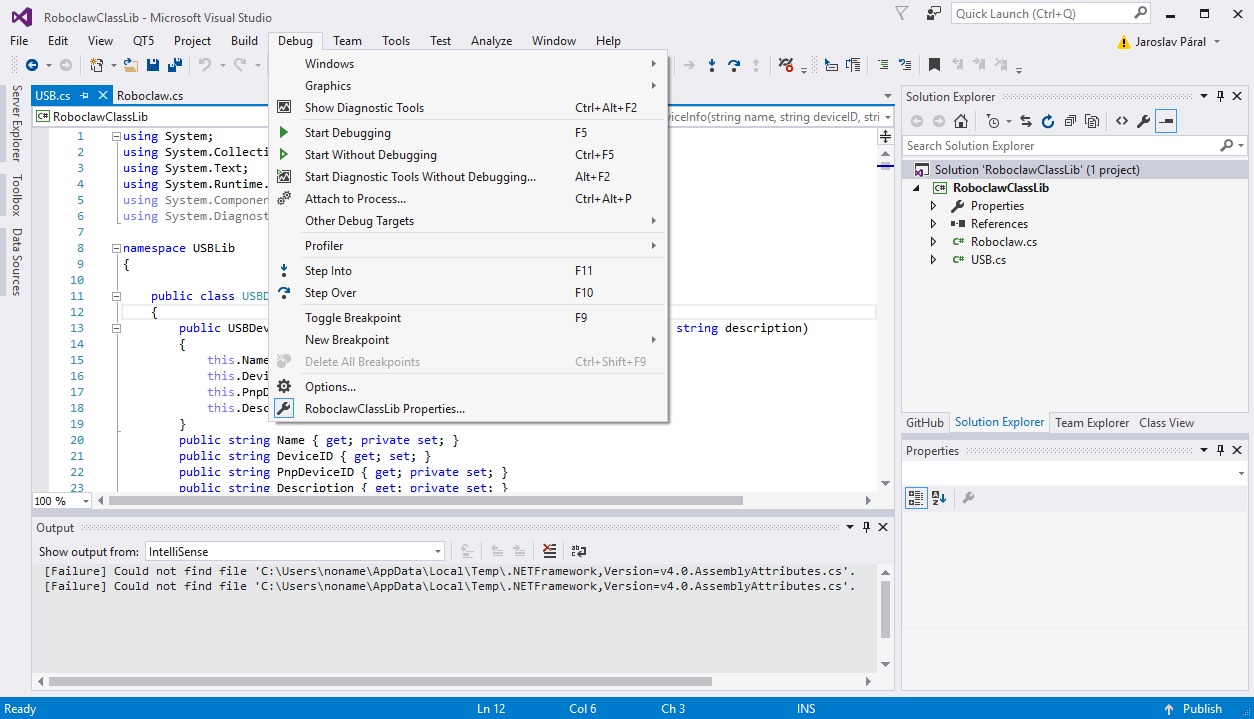
\includegraphics[width=\textwidth]{images/visual-studio_debug.png}
    \caption[Ukázka prostředí v~Microsoft Visual Studio Community 2015]{Ukázka prostředí v~Microsoft Visual Studio Community 2015 \\
    Aby uživatel spustil program, musí vybrat volbu \texttt{Start Without Debugging}, což je v~pořadí až druhá volba a~začátečník ani nemusí tušit, co znamená slovo debugging. 
    }
    \label{fig:visual-studio-community-2015}
\end{figure}

\begin{figure}[h]
    \centering
    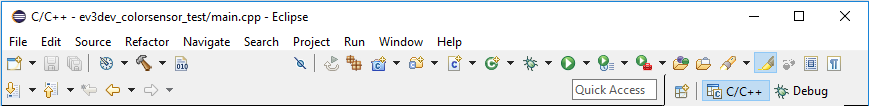
\includegraphics[width=\textwidth]{images/eclipse_tools-panel_focus.png}
    \caption[Ukázka panelu nástrojů v~prostředí Eclipse]{Ukázka panelu nástrojů v~prostředí Eclipse \\
    Zkuste vysvětlit skupině 15 začátečníků, kterou ikonku mají zmáčknout pro překlad, a~kterou pro spuštění. S~velkou pravděpodobností to polovina udělá poprvé špatně.  
    }
    \label{fig:eclipse_tools-panel}
\end{figure}

\subsection{Arduino IDE a~Processing}



Na opačné straně vývojářských nástrojů stojí programy Arduino IDE~\cite{arduino-web} a~Processing~\cite{processing-web} (stále kategorie~C).

Arduino IDE je vývojářský nástroj pro open-source elektronickou platformu Arduino, s~kterou lze jednoduše sestavovat hardware a~programovat software.
To vše bez potřeby drahého vybavení a~hlubších znalostí programování a~mikroprocesorů. 
Platforma využívá převážně mikrokontroléry AVR od firmy Atmel.
Jako programovací jazyk se používá Wiring~\cite{arduino-wiring}, který vychází z~jazyka C.

Processing je taktéž open-source vývojářský program, ale i~jazyk, určený pro snadnou tvorbu vizuálně zajímavé a~interaktivní grafiky.
Vznikl v~rámci MIT Media Lab~\cite{processing-web_overview} jako nástroj pro umělce a~lidi, kteří chtějí tvořit elektronické umění, ale nejsou programátoři.
Proto bylo hlavním cílem vytvořit jednoduché prostředí, které jim to umožní. Jazyk Processing je postaven nad Javou.

Arduino na Processing navázalo a~snaží se tuto myšlenku rozšířit na hardware. 
Zároveň použilo vývojářský program od Processingu a~upravilo jej pro své potřeby. 
V~mnoha oblastech se tyto dva projekty doplňují. 
Například lze pomocí Processingu graficky vizualizovat naměřené hodnoty ze senzorů připojených k~Arduinu.

Podle mého názoru nabízejí začátečníkovi přesně to co potřebuje: jednoduché UI, v~kterém se rychle zorientuje a~hned najde základní komponenty potřebné k~práci (hlavně tlačítka pro překlad a~spuštění programu). 
Vše si lze prohlédnout na obrázcích~\ref{fig:arduino+processing} a~\ref{fig:arduino-ide_tools-panel}.

\begin{figure}[h]
    \centering
    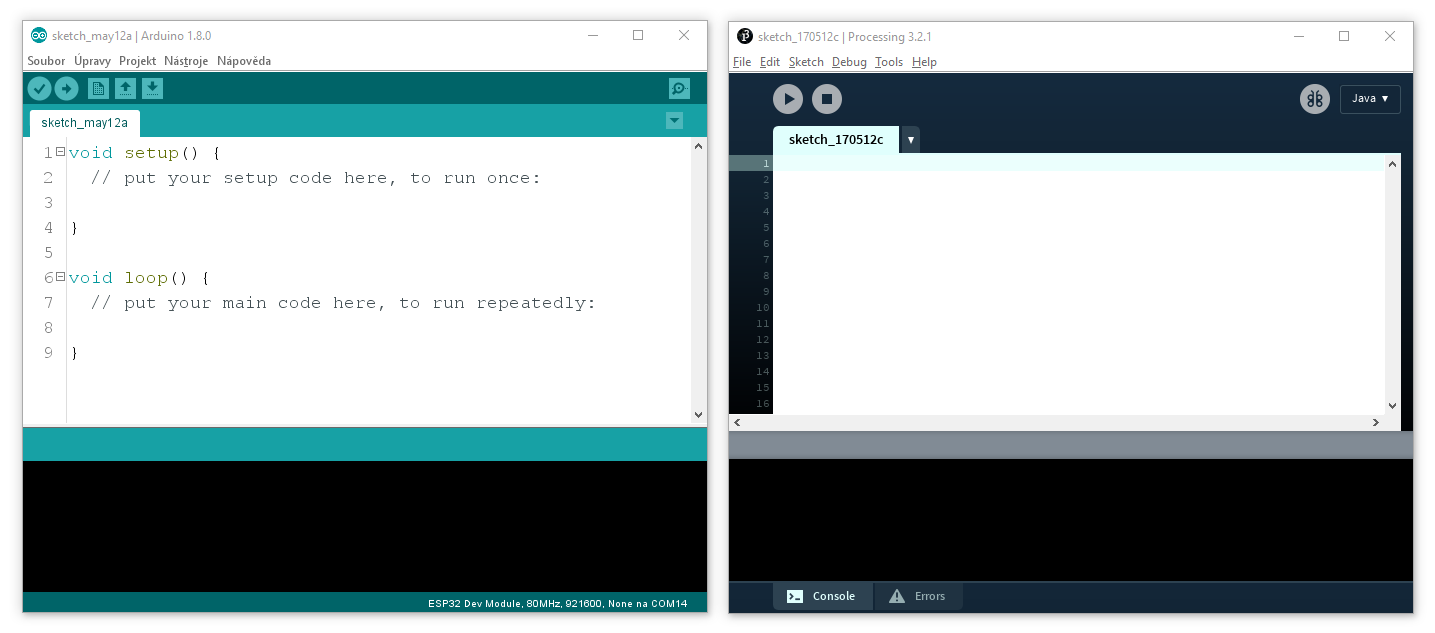
\includegraphics[width=\textwidth]{images/arduino+processing.png}
    \caption[Ukázka jednoduchých prostředí Arduino IDE a~Proccessing]{Ukázka jednoduchých prostředí Arduino IDE a~Proccessing \\
    Základní ovládací prvky potřebné při vývoji programů (tlačítka pro přeložení a~spuštění programu) jsou jasně a~zřetelně na očích a~neztrácejí se v~mnoha dalších ikonkách.}
    \label{fig:arduino+processing}
\end{figure}

\begin{figure}[h]
    \centering
    
\includegraphics[width=\textwidth]{images/arduino-ide_tools-panel.png}
    \caption{Panel s~nástroji v~Arduino IDE -- uživatel zde hned najde vše, co potřebuje}
    \label{fig:arduino-ide_tools-panel}
\end{figure}

I~tyto programy mají ale své problémy. 
Arduino IDE neumí našeptávat nebo zobrazovat nápovědu k~funkcím. 
Zároveň špatně zobrazuje chybové hlášky objevené při překladu.

Processing je na tom lépe. 
Má integrovaný základní našeptávač. 
Dokonce zvládá ukazovat datové typy parametrů.
Nezobrazuje však už jejich název, tudíž většinou nelze určit, co za parametr se očekává.
Lépe je v editoru zapracováno i~vypisování chyb a~je možné zapnout i~kontrolu správnosti kódu v průběhu psaní.

Bohužel tato IDE jsou šitá na míru daným platformám a~proto je nelze v~rámci mé práce využít. 

Poslouží ale jako dobrá inspirace pro výběr vhodného editoru.

\subsection{Visual Studio Code}


Po vyzkoušení výše zmíněných IDE jsem se rozhodl vrátit ke~kategorii~B a vyzkoušet nový editor Visual Studio Code. 
Jedná se o~relativně čerstvý počin Microsoftu, který tento editor představil v~rámci BUILDu 2015~\cite{visual-studio-code_initial-release}.


Visual Studio Code (dále jen VS Code) je zdarma dostupný multiplatformní (Windows, Linux, Mac) open-source editor s~integrovaným našeptáváním, Gitem a~podporou doplňků a~skriptování.
Probíhá u~něj velmi rychlý vývoj a~aktuálně jej lze považovat za jeden z~nejlepších editorů v~této kategorii.
V mnoha ohledech již předčil své konkurenty (editor Atom a~Sublime).
Například ve~srovnání s~Atomem je výrazně rychlejší.

Oproti vývojovým IDE z~kategorie~C má dle mého názoru značně jednoduší UI, při zachování rozsáhlých možností rozšiřování a~pokročilých funkcí. 
Základní funkce jsou dostupné přes nabídku v~horní a~boční liště. 
Všechny ostatní funkce lze najít přes speciální příkazovou řádků, která se spouští klávesovou zkratkou \texttt{Ctrl+Shift+P}. 
Tato příkazová řádka je ale běžnému uživateli skrytá a~tak jej neruší při používání.
Díky tomu nabízí VS~Code velké množství funkci při zachování jednoduchého uživatelského rozhraní.

\begin{figure}[h]
    \centering
    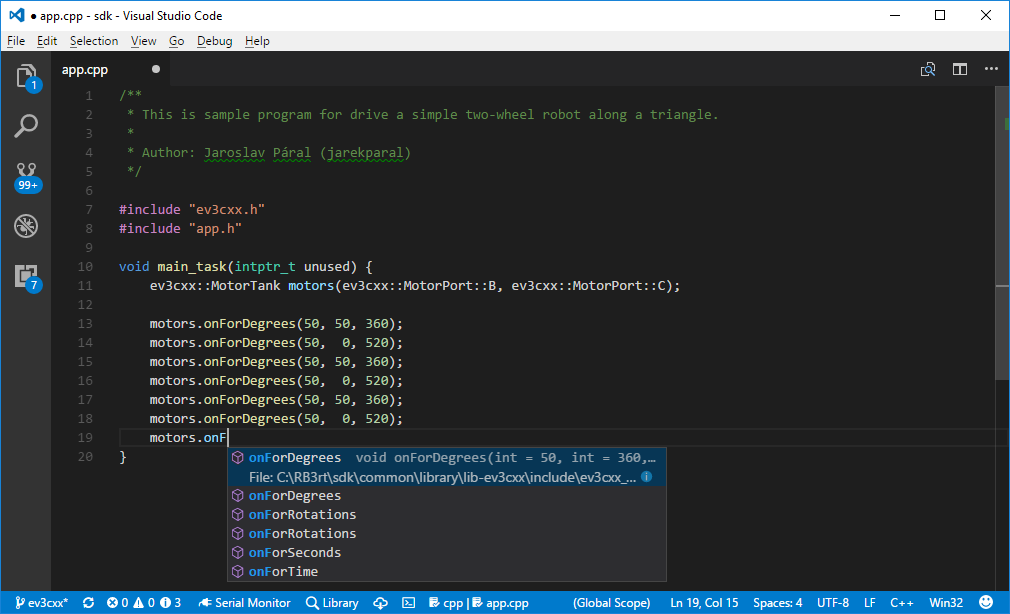
\includegraphics[width=\textwidth]{images/visual-studio-code_intellisense-function.png}
    \caption{Ukázka našeptávání ve Visual Studio Code -- doplňování názvu funkce}
    \label{fig:visual-studio-code_intellisense-function}
\end{figure}


Do VS~Code je možné nainstalovat celou řadu rozšíření. 
Tím nejzajímavější je doplněk  \texttt{C/C++ for Visual Studio Code}~\cite{vs-code_cpptools} přímo od~Microsoftu, který nabízí velmi dobré našeptávání, automatické formátování nebo vyhledávání definic a~symbolů.
Tato funkcionalita například velmi chybí v~Arduino IDE, na což si většina mých studentů v~kurzech stěžuje, když zjistí, že ji jiný nástroj umí.

Dalšími důležitými funkcemi jsou integrovaný terminál a~možnost jednoduchého spouštění skriptů.
VS~Code také nabízí snadné nadefinování klávesových zkratek, s~jejichž pomocí lze volat vlastní skripty.
Touto cestou jsem se rozhodl implementovat překlad uživatelských programů a~následné zasílání programu do~EV3.
K veškeré činnosti uživateli stačí jen tři klávesové zkratky: přeložení programu, odeslání programu a~kombinace předchozích dvou příkazů v~rámci jedné klávesy. 